\section{Manejando otros Problemas en lineales regresión}

Hasta ahora en este capítulo, hemos aprendido:
\begin{itemize}
	\item Cómo implementar un modelo de regresión lineal usando dos métodos
	\item Cómo medir la eficiencia del modelo usando los parámetros del modelo
\end{itemize}


Sin embargo, hay otros Problemas que deben tenerse en cuenta al tratar con fuentes de datos de diferentes tipos. Repasemos uno por uno. Usaremos un diferente conjunto de datos simulado para ilustrar estos Problemas. Vamos a importarlo y echarle un vistazo
en eso:

[,]{\texttt{handlingIssues.py}}
\begin{lstlisting}[language=Python]
	import pandas as pd
	df=pd.read_csv('./dataBases/EcomExpense.csv')
	print(df.head())
\end{lstlisting}

[,]{}
Deberíamos obtener los siguientes resultados:

\begin{lstlisting}[language=Python]
	Transaction ID  Age    Items   Monthly Income  Transaction Time  Record  \
	0         TXN001    42       10            7313        627.668127       5
	1         TXN002    24        8           17747        126.904567       3
	2         TXN003    47       11           22845        873.469701       2
	3         TXN004    50       11           18552        380.219428       7
	4         TXN005    60        2           14439        403.374223       2
	
	Gender City Tier  Total Spend
	0  Female    Tier 1  4198.385084
	1  Female    Tier 2  4134.976648
	2    Male    Tier 2  5166.614455
	3  Female    Tier 1  7784.447676
	4  Female    Tier 2  3254.160485
\end{lstlisting}

[]{}
La captura de pantalla anterior es un conjunto de datos simulados del sitio web de cualquier comercio. Esto captura la información sobre varias transacciones realizadas en el sitio web.


Una breve
La descripción de los nombres de columna del conjunto de datos es la siguiente:
\begin{itemize}
	\item Identificación de transacción: ID de transacción para la transacción
	\item Edad: Edad del cliente
	\item Artículos: número de artículos en el carrito de compras (comprado)
	\item Ingreso mensual: Ingreso disponible mensual del cliente
	\item Tiempo de transacción: tiempo total pasado en el sitio web durante la transacción
	\item Registro: cuántas veces el cliente ha comprado con el sitio web en
	el pasado
	\item Género: Género del cliente
	\item Nivel de la ciudad: ~
	\item Gasto total: monto total gastado en la transacción
\end{itemize}



La variable de salida es la variable\texttt{Total Spend (Gasto total)}. Los otros son predictores potenciales
variables y sospechamos que el gasto total está relacionado linealmente con todos estos
variables predictoras.


\subsection{Manejando variables categóricas}

Hasta ahora, hemos supuesto que las variables de predicción solo pueden ser cuantitativas o
numéricas, pero sabemos por experiencias de la vida real que la mayoría de las veces \emph{el conjunto de datos
	contiene una variable categórica o cualitativa} y muchas de las veces estas variables
tendrá un impacto significativo en el valor de la salida. Sin embargo, la pregunta es
\emph{¿cómo procesar estas variables, para usarlas en el modelo?}


No podemos asignarles valores, como 0, 1, 2, etc., y luego usarlos en el
modelo, ya que dará un peso excesivo a las categorías debido a los números
asignado a ellos. 

La mayoría de las veces puede dar un resultado incorrecto y cambiará,
como cambia el número asignado a una categoría en particular.


En el marco de datos que acabamos de importar, Género y Nivel de ciudad son los categóricos
variables.


Para manejar variables categóricas, usaremos variables ``tontas'' (dummies, en inglés) o ficticias.


Una regresión lineal es de la forma
\begin{align}
	Y_{\texttt{model}}=\a + \sum \beta_{i}X_{i}
\end{align}
en la cual algunas $X_{i}$ pueden ser categóricas. Digamos que $X_{g}$ es tal variable.


En nuestro ejemplo,
\begin{align}X_{g}=
	\begin{cases}
		1 & \texttt{cliente masculino} \\
		0 & \texttt{cliente femenino}
	\end{cases}
\end{align}


Si hay tres niveles en la variable categórica, entonces uno necesita definir dos
variables en comparación con 1 cuando había dos niveles en la variable categórica.

Por ejemplo, la variable \texttt{City Tier} tiene tres niveles en nuestro conjunto de datos.


Para esto, podemos definir dos variables, tales que:
\begin{align}
	X_{t1}=
	\begin{cases}
		1 & \texttt{``City Tier''}=1 \\
		0 & \texttt{``City Tier''}\neq 1
	\end{cases}
\end{align}
\begin{align}
	X_{t2}=
	\begin{cases}
		1 & \texttt{``City Tier''}=2 \\
		0 & \texttt{``City Tier''}\neq 2
	\end{cases}
\end{align}


Entonces, el modelo puede ser alguno de los siguientes
\begin{align}
	Y=
	\begin{cases}
		\a + \beta_{1}X_{1}+...+\beta_{t1}X_{t1}+...+b_{n}X_{n} & \texttt{``City Tier''=1}\\
		\a + \beta_{1}X_{1}+...+\beta_{t1}X_{t2}+...+b_{n}X_{n} & \texttt{``City Tier''=2}\\
		\a + \beta_{1}X_{1}+...++b_{n}X_{n} & \texttt{``City Tier''=3}\\
	\end{cases}
\end{align}


Tengan en cuenta que uno no tiene que crear la tercera variable. Esto es
debido a la naturaleza en que se definen estas variables.


Si un
el cliente no pertenece a la ciudad de nivel 1 o nivel 2, entonces ciertamente lo hará
pertenece a una ciudad de nivel 3. Por lo tanto, no se requiere una variable para uno de
los niveles.


\begin{observacion}
	En general, para variables categóricas que tienen $n$ niveles, uno
	debería crear $(n-1)$ variables ficticias.
\end{observacion}

Sin embargo, por simplicidad, utilizaremos cada uno de los niveles.


Creemos ahora las variables ficticias para nuestras
variables categóricas y luego agreguémoslas a nuestro marco de datos, como se muestra:


[,]{}

\begin{lstlisting}[language=Python]
	dummy_gender=pd.get_dummies(df['Gender'],prefix='Sex')
	dummy_city_tier=pd.get_dummies(df['City Tier'],prefix='City')
\end{lstlisting}


Veamos cómo se ven y si satisfacen las condiciones que hemos definido
antes o no. Así es como se ve \texttt{dummy\_city\_tier}:

[,]{}
\begin{lstlisting}[language=Python]
	City_Tier 1  City_Tier 2  City_Tier 3
	0            1            0            0
	1            0            1            0
	2            0            1            0
	3            1            0            0
	4            0            1            0
\end{lstlisting}

[,]{}
\texttt{dummy\_gender} es similar a la siguiente tabla:
\begin{lstlisting}[language=Python]
	Sex_Female  Sex_Male
	0           1         0
	1           1         0
	2           0         1
	3           1         0
	4           1         0
\end{lstlisting}


Ahora, tenemos estas variables ficticias creadas pero no son parte del
marco principal de datos todavía. Vamos a adjuntar estas nuevas variables al marco de datos principal para que
se puede usar en el modelo:

[,]{}

\begin{lstlisting}[language=Python]
	Transaction ID  Age    Items   Monthly Income  Transaction Time  Record  \
	0         TXN001    42       10            7313        627.668127       5
	1         TXN002    24        8           17747        126.904567       3
	2         TXN003    47       11           22845        873.469701       2
	3         TXN004    50       11           18552        380.219428       7
	4         TXN005    60        2           14439        403.374223       2
	
	Gender City Tier  Total Spend  Sex_Female  Sex_Male  City_Tier 1  \
	0  Female    Tier 1  4198.385084           1         0            1
	1  Female    Tier 2  4134.976648           1         0            0
	2    Male    Tier 2  5166.614455           0         1            0
	3  Female    Tier 1  7784.447676           1         0            1
	4  Female    Tier 2  3254.160485           1         0            0
	
	City_Tier 2  City_Tier 3
	0            0            0
	1            1            0
	2            1            0
	3            0            0
	4            1            0
\end{lstlisting}


Hay cinco nuevas columnas en el marco de datos, dos de las variables ficticia de \texttt{Gender} y tres de las variables ficticias de \texttt{City Level}.


Si lo compara con el conjunto de datos completo, \texttt{City\_Tier\_1} tiene el valor 1 si \texttt{City\_Tier}
tiene valor de \texttt{Tier 1}, \texttt{City\_Tier\_2} tiene valor 1 si \texttt{City\_Tier} tiene valor de \texttt{Tier 2} y
\texttt{City\_Tier\_3} tiene valor 1 si \texttt{City\_Tier} tiene valor \texttt{Tier 3}. Todas las demás variables ficticias en esa fila particular tendrán valores 0. Esto es lo que queríamos.


Veamos cómo incluir estas variables ficticias en el modelo y cómo evaluarlas
sus coeficientes.

Para el conjunto de datos anterior, supongamos una relación lineal entre la salida
variable de Gasto Total y las variables predictoras: \texttt{Ingreso Mensual} y
\texttt{Tiempo de transacción}, y ambos conjuntos de variables ficticias:

[,]{}

\begin{lstlisting}[language=Python]
	from sklearn.linear_model import LinearRegression
	feature_cols = ['Monthly Income','Transaction Time','City_Tier 1',\
	'City_Tier 2','City_Tier 3','Sex_Female','Sex_Male']
	X = df2[feature_cols]
	Y = df2['Total Spend']
	lm = LinearRegression()
	lm.fit(X,Y)
\end{lstlisting}

[,]{}
Los parámetros del modelo se pueden encontrar de la siguiente manera:
\begin{lstlisting}[language=Python]
	print(lm.intercept_)
	for _ in zip(feature_cols, lm.coef_):
	print(_)
\end{lstlisting}

[,]{}
\begin{lstlisting}[language=Python]
	3655.72940769
	('Monthly Income', 0.15297824609320512)
	('Transaction Time', 0.12372608642619998)
	('City_Tier 1', 119.66325160390086)
	('City_Tier 2', -16.67901800799039)
	('City_Tier 3', -102.9842335959104)
	('Sex_Female', -94.157798830320132)
	('Sex_Male', 94.157798830320118)
\end{lstlisting}

[,]{}
El valor $R^2$ para este modelo se puede encontrar escribiendo lo siguiente:
\begin{lstlisting}[language=Python]
	R2 = lm.score(X,Y)
	print(R2)
	## 0.194789205529
\end{lstlisting}


El valor resulta ser $0.19$, lo que podría deberse a que no hemos usado las otras variables y el resultado también podrían estar relacionados con ellos. 

Necesitamos ajustar el
modelo al transformar adecuadamente algunas de las variables y agregarlas al modelo. 

Por ejemplo, si agregamos la variable \texttt{Record} al modelo, $R^2$ salta a $0.91$ (intente eso
por su cuenta). Es un buen conjunto de datos para jugar.

El modelo se puede escribir de la siguiente manera:
\begin{align}
	\texttt{Total\_Spend}= & 3655.72+0.12*\texttt{Transaction Time} \\ &+0.15*\texttt{Monthly Income}+119*\texttt{City\_Tier 1}\\
	& -16*\texttt{City\_Tier 2} - 102*\texttt{City\_Tier 3}\\
	& -94*\texttt{Sex\_Female}+94*\texttt{Sex\_Male}
\end{align}

[,]{}
El RSE se puede calcular de la siguiente manera:

\begin{lstlisting}[language=Python]
	import numpy as np
	df2['total_spend_pred']=3720.72940769 + 0.12*df2['Transaction Time']+ \
	0.15*df2['Monthly Income']+119*df2['City_Tier 1']-16*df2['City_Tier 2']
	-102*df2['City_Tier 3']-94*df2['Sex_Female']+94*df2['Sex_Male']
	df2['RSE']=(df2['Total Spend']-df2['total_spend_pred'])**2
	RSEd=df2.sum()['RSE']
	RSE=np.sqrt(RSEd/2354)
	salesmean=np.mean(df2['Total Spend'])
	error=RSE/salesmean
	print(RSE,salesmean,error)
	##2518.85203887 6163.176415976714 0.408693808008
\end{lstlisting}


Para diferentes niveles de género y ciudad, el modelo se reducirá a seguir para
diferentes casos:
\begin{center}
	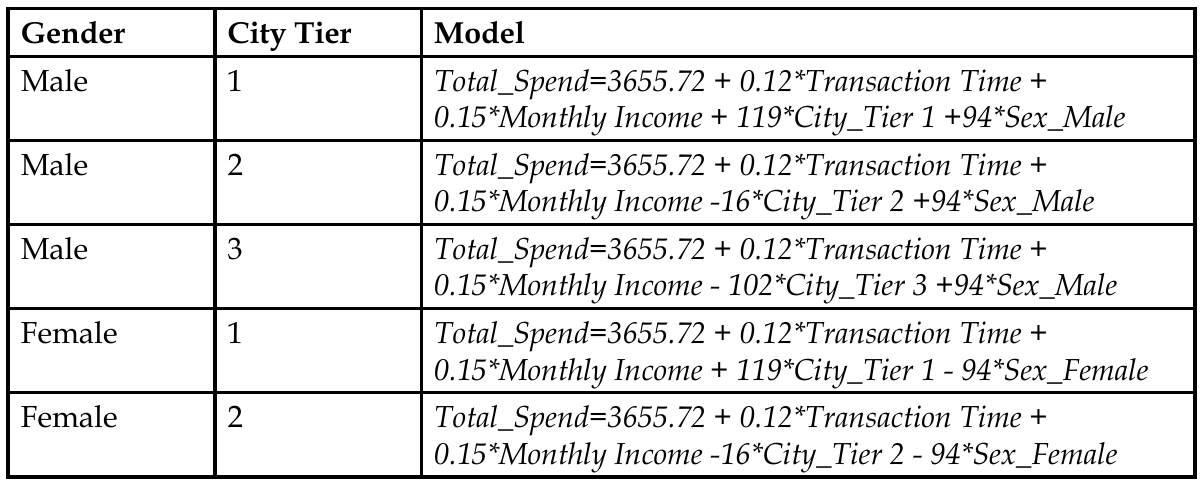
\includegraphics[width=10cm,keepaspectratio=true]{./images/dummies.png}
	% dummies.png: 0x0 pixel, 300dpi, 0.00x0.00 cm, bb=
\end{center}



\subsection{Transformando una variable para ajustarla a una relación no lineal}

A veces, la variable de salida no tiene una relación lineal directa con el
variable de predicción, es decir, tienen una relación no lineal.


Estas relaciones podrían
funciones simples como cuadrática, exponencial, logaritmo o complejas como
polinomios. En tales casos, la transformación de la variable es muy útil.


La siguiente es una guía aproximada sobre cómo hacerlo:
\begin{enumerate}
	\item
	Trace un diagrama de dispersión de la variable de salida con cada uno de los predictores
	variables. Este se puede pensar como una matriz de diagrama de dispersión similar a
	la matriz de correlación
	\item Si la gráfica de dispersión asume más o menos una forma lineal para una variable de predicción
	entonces está relacionado linealmente con la variable de salida.
	\item Si el diagrama de dispersión asume una forma característica de diferente de la lineal para una variable de predicción, entonces transformaremos esa variable en particular
	aplicando esa función.
\end{enumerate}


Vamos a ilustrar esto con un ejemplo. Usaremos el conjunto de datos \texttt{Auto.csv} para esto.
Este conjunto de datos contiene información sobre millas por galón (mpg) y caballos de fuerza para
una serie de modelos de automóviles y mucho más. El \texttt{mpg} es la variable de predicción y es
considerado altamente dependiente de la potencia de un modelo de automóvil.

[,]{\texttt{nonLinear.py}}
\begin{lstlisting}[language=Python]
	import pandas as pd
	data = pd.read_csv('./dataBases/Auto.csv')
	print(data.head())
\end{lstlisting}

[,]{}

\begin{lstlisting}[language=Python]
	mpg  cylinders  displacement  horsepower  weight  acceleration  \
	0  18.0          8         307.0       130.0    3504          12.0
	1  15.0          8         350.0       165.0    3693          11.5
	2  18.0          8         318.0       150.0    3436          11.0
	3  16.0          8         304.0       150.0    3433          12.0
	4  17.0          8         302.0       140.0    3449          10.5
	
	model year  origin                   car name
	0          70       1  chevrolet chevelle malibu
	1          70       1          buick skylark 320
	2          70       1         plymouth satellite
	3          70       1              amc rebel sst
	4          70       1                ford torino
\end{lstlisting}


Tiene 406 filas y 9 columnas. Algunas de las variables tienen valores de \texttt{NA (not available)} y tiene sentido eliminar los valores \texttt{NA} antes de usarlos.

[,]{}
Ahora, tracemos un diagrama de dispersión entre las variables de potencia y \texttt{mpg} para ver
ya sea que exhiban una forma lineal o alguna forma no lineal:
\begin{lstlisting}[language=Python]
	import matplotlib.pyplot as plt
	#%matplotlib inline
	data['mpg']=data['mpg'].dropna()
	data['horsepower']=data['horsepower'].dropna()
	plt.plot(data['horsepower'],data['mpg'],'ro')
	plt.xlabel('Horsepower')
	plt.ylabel('MPG (Miles Per Gallon)')
\end{lstlisting}


\begin{figure}
	\centering
	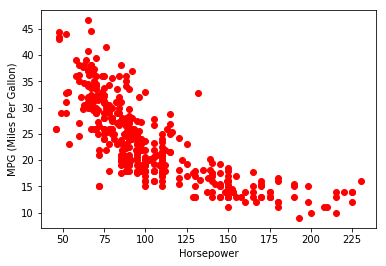
\includegraphics[width=10cm,keepaspectratio=true]{./images/hpVsMpg.png}
	% hpVsMpg.png: 0x0 pixel, 300dpi, 0.00x0.00 cm, bb=
	\caption{\texttt{HP vs MPG}}
	\label{fig:hp}
\end{figure}


Aunque hemo supuesto que el modelo es lineal
\begin{align}
	mpg = c_{0} + c_{1}*\texttt{hp}
\end{align}
en realidad parece más un \emph{modelo cuadrático}
\begin{align}
	mpg = c_{0} + c_{1}*\texttt{hp} + c_{2}\texttt{hp}^{2}
\end{align}


El siguiente fragmento de código se ajustará a un modelo lineal entre potencia y mpg
variables. Los valores de NA deben eliminarse de las variables antes de que puedan
ser utilizado en el modelo. También simultáneamente, creemos un modelo asumiendo un lineal
relación entre mpg y cuadrado de potencia:

[,]{}
\begin{lstlisting}[language=Python]
	import numpy as np
	from sklearn.linear_model import LinearRegression
	X=data['horsepower'].fillna(data['horsepower'].mean())
	Y=data['mpg'].fillna(data['mpg'].mean())
	lm=LinearRegression()
	lm.fit(X[:,np.newaxis],Y)
\end{lstlisting}


El método de regresión lineal por defecto requiere que X sea una matriz de dos
dimensiones. Usando \texttt{np.newaxis}, estamos creando una nueva dimensión para que
funcione correctamente.

La línea de mejor ajuste se puede trazar con el siguiente fragmento:

[,]{}
\begin{lstlisting}[language=Python]
	import matplotlib.pyplot as plt
	%matplotlib inline
	plt.plot(data['horsepower'],data['mpg'],'ro')
	plt.plot(X,lm.predict(X[:,np.newaxis]),color='blue')
\end{lstlisting}



\begin{center}
	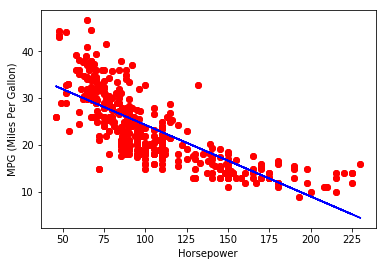
\includegraphics[width=10cm,keepaspectratio=true]{./images/hpLR.png}
	% hpLR.png: 0x0 pixel, 300dpi, 0.00x0.00 cm, bb=
\end{center}
[,]{}
\begin{lstlisting}[language=Python]
	R2 = lm.score(X[:,np.newaxis],Y)
	print(R2)
	## 0.574653340645
	
	RSEd=(Y-lm.predict(X[:,np.newaxis]))**2
	RSE=np.sqrt(np.sum(RSEd)/389)
	ymean=np.mean(Y)
	error=RSE/ymean
	print(RSE,error)
	## 5.1496254787 0.21899719414
\end{lstlisting}


Aquí, estamos usando el método \texttt{predict} para calcular el valor predicho de la
modelo en lugar de escribirlos explícitamente.

El valor de RSE para este modelo resulta ser 5.14, que sobre un valor medio de 23.51 da un error del 21\%



Si el modelo es cuadrático, esto se puede ajustar utilizando el método \texttt{PolynomialFeatures} en la biblioteca \texttt{scikit-learn}. En este modelo, asumimos una relación polinómica entre mpg
y caballos de fuerza:

[,]{\texttt{nonLinear.py}}
\begin{lstlisting}[language=Python]
	from sklearn.preprocessing import PolynomialFeatures
	from sklearn import linear_model
	X=data['horsepower'].fillna(data['horsepower'].mean())
	Y=data['mpg'].fillna(data['mpg'].mean())
	poly = PolynomialFeatures(degree=2)
	X_ = poly.fit_transform(X[:,np.newaxis])
	clf = linear_model.LinearRegression()
	clf.fit(X_, Y)
	
	print(clf.intercept_)
	##55.0261924471
	print(clf.coef_)
	##[ 0.         -0.43404318  0.00112615]
\end{lstlisting}


El modelo se puede escribir entonces como
\begin{align}
	\texttt{mpg}  = 55.02 -0.43*\texttt{hp}+0.001*\texttt{hp}^{2}
\end{align}

[,]{}
Con el siguiente fragmento de código, podemos visualizar el modelo cuadrático:
\begin{lstlisting}[language=Python]
	plt.plot(data['horsepower'],data['mpg'],'ro')
	plt.plot(X,clf.predict(X_), "bo")
	plt.show()
\end{lstlisting}


\begin{center}
	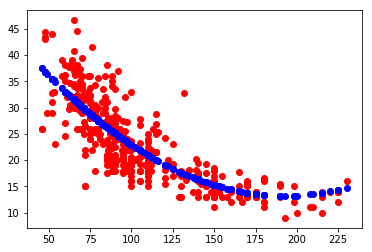
\includegraphics[width=10cm,keepaspectratio=true]{./images/hpNLR.png}
	% hpNLR.png: 0x0 pixel, 300dpi, 0.00x0.00 cm, bb=
\end{center}


